%===================================== CHAP 4 =================================

\chapter{Experiment}

\todo{Give an overview of the experiment first.}
Introduce the experiment

\section{Dataset}
This section will introduce the dataset(s) used. What features it contains, what we try to learn/classify, and why we chose to use it.
The Spambase Dataset \cite{spambase1999data} was used as a baseline training set. This dataset is publicly available from the UCI machine learning directory, and contains 57 input attributes of continuous format which serves as input features for spam detection and 1 target attribute in discrete format which represents the class.

We chose this dataset as it is a popular dataset to analyze the performance of binary classifiers, so that we could compare the results of other logistic regression classifiers against our own. While this dataset might not seem like the ideal choice for testing a differentially private classifier due to its lack of personal information, we argue that it still fits well for the purpose of demonstration. In a spam-classifying system based on our distributed model, a logistic regression model can be built by training it locally in each user's personal mail folder and then aggregated into an ensemble. That way you can build a diverse spam-classifier without the users having to give up their personal email to a centralized database.     

Used normalization to scale the data to 0-1 range, this is due to the proof in Chaudhuri paper which states the assumption $|X_i|< 1$. Based on the formula
\begin{eqnarray}
	X_{norm} = \frac{X-X_{min}}{X_{max} - X_{min}}
\end{eqnarray}

We appended a feature with constant value 1.0 to all data records, to act as the intercept or bias term. 

\section{Parameter tuning}
\label{sec:parameter_tuning}
Number of peers $P$ specifies how many different peers participate in the experiment, and necessarily the number of partitions of the training data sets. The training is divided into $P$ parts of equal size.

\todo[inline]{Rationalize why we have included 1 in the 10-inteval experiments - it is because 1 is a very interesting edge case. Should also talk about the significance of group size 1  in analysis.}

Aggregate models are created from local models at each peer through an aggregation process that is performed one or more times with subsets of peers. The parameter $g$ specifies how many peers will participate in a single model aggregation. Since each peer has a unique subset of data, this parameter determines how many partitions of the training set contribute to the published aggregate models. These data partitions do not contribute directly, but indirectly through the aggregation of models trained locally on each partition.

Each peer trains a local logistic regression classifier on its data partition. This requires selection of a learning rate $\alpha$, a regularization constant $\lambda$ and a maximum number of iterations of gradient descent $I$. The learning rate is sensitive to the size of the local training set\cite{wilson20013learningrate}, and should be tuned individually by each peer. We did this by running 3-fold cross validation when each peer fits its local model to identify the best $\alpha$ in the range $[-7, 0]$. 3-fold cross validation was chosen because of both project computer time constraints and experimental data constraints. Each experiment in its entirety is tested with 10-fold cross validation, so it was necessary to reduce local model training time in order to run in a reasonably short time on a single computer. The data constraints is a part of the domain we want to explore. When the amount of data is very small, 3-fold cross validation offers a balance between parameter search reliability and validation set sizes.

In usual data mining applications the regularization $\lambda$ would be tuned in this manner as well, but the sensitivity of the aggregation mechanism depends on $\lambda$, as seen in Equation \ref{eq:aggregated_logistic_sensitivity}. This means that the peers will have to communicate to either agree on a regularization level or to determine the smallest regularization constant to identify the worst case noise level. In our experiments we chose a global regularization level, which was used by all peers. We identified the best $\lambda$ by testing a coarse grid of powers of 2 whenever we changed the per-peer number of training samples. \todo[inline]{Explain the specific way of how regularization was establish. Probably: whenever number of peers changed, we ran an experiment over regularization with other parameters fixed to constant values. Explain why this is okay. We should also discuss possible problems with this.}

\todo[inline]{Explain why we are doing the inital test with a range of regularization. Essentially, it is because epsilon can be seen as fixed, learning rate is found by CV and lambda is the only remaining parameter that is essentialy to tuning the performance of individual models.]}

\todo{Talk about the problem of tuning regularization. We are essentially doing a global selection of regularization. This could be difficult. Better to communicate the minimum, perhaps? But then, which regularization should peers pick locally? The highest one that stil has good performance?}

The privacy parameter $\epsilon$ determines the level of privacy for each data partition. Note that this parameter does not apply to the original training set as a whole - each peer has its own private database, which is protected by $\epsilon$-differential privacy. 

Finally, the parameter $\epsilon$ can be divided across several applications of the aggregation mechanism, as described in Section \ref{section:privacy_budget}. This was achieved with a per-aggregation parameter $\epsilon_i$. Each data partition can participate the aggregation mechanism $n$ times, where $n\epsilon_A \leq \epsilon$.

\todo{Insert logistic regression training algorithm including hyperparameter usage}

\section{Validation}

The test sets set aside could not be used when tuning and evaluating system hyperparameters. In order to explore the effects of the various hyperparameters we used cross validation with number of folds $n=10$. For a given combination of hyperparameters, performance metrics were measured as their average across ten repetitions. In repetition $i$, data fold $i$ was used as validation set and the remaining $n-1$ data folds were combined to form the test set.

For the XXXX experiment\todo{insert experiment here}, the test set was used.

\section{Algorithm}

This section explain the logistic regression algorithm, how it is commonly used, and what modifications are needed when used in a distributed setting. Explanation on how it is used in a differentially private manner is explained in the architecture section. 

\subsection{Platform Setup}

\subsection{Application of Aggregation Mechanism}



The central element in our experiments is the aggregation mechanism $A$, which takes a set of models. This mechanism is given in Algorithm \ref{alg:privacy_mechanism}. As presented in Section \ref{sec:Sensitivity_of_LogReg}, the sensitivity of logistic regression depends on the sizes of the data sets used to train the models. Specifically, the mechanism needs to know the size of the smallest training set in order to guarantee differential privacy. It is important to note that the method we are testing assumes honest-but-curious participants, as assumed by Pathak et al\cite{pathak2010diffprivhomo}.

\begin{algorithm}[H]
	\label{alg:privacy_mechanism}
		\KwIn{$\epsilon$ - privacy parameter
			$\boldmath{M}$ - set of models trained by participating peers\;
			$\boldmath{N}$ - set of peer training set sizes\;
			$\lambda$ - regularization level used when training each model in $\boldmath{M}$\;
			}
		\KwOut{Perturbed aggregate of the models in $\boldmath{M}$}
		$n_{min} \leftarrow min(\boldmath{N})$\;
		$\eta \leftarrow Laplace(0; \frac{2}{n_{min}\epsilon\lambda})$\;
		$model_{agg} \leftarrow 1/K\sum_{j=1}^{|\boldmath{N}|} \boldmath{w_j} + \boldmath{\eta}$\;
		\KwRet{$model_{agg}$}
		
\caption{$\epsilon$-differentially private aggregation mechanism}
\end{algorithm}

\begin{algorithm}[H]
	\KwIn{$P$ - the set of peers\;
		$\epsilon$ - privacy parameter\; 
		$\epsilon_A$ - privacy level of a mechanism application\;
		$A$ - the $\epsilon_A$-differentially private aggregation mechanism\;
		$group\_size$ - number of peers in a single mechanism application}
	\For{peer $\in$ P}{
		$budget_{peer} \leftarrow \epsilon$\;
	}
	\While{$|P| \geq group\_size$}{
		$group \leftarrow randomSample(P, group\_size)$\;
		$model_{agg} \leftarrow A(group)$\;
		\For{peer $\in$ group}{
			$budget_{peer} \leftarrow budget_{peer} - \epsilon_A$\;
			\If{$budget_{peer} < \epsilon_A$}{
				$P \leftarrow P \smallsetminus peer$\;
			}
		}
		$publish(P, model_{agg})$
}
\caption{Application of aggregation mechanism}
\end{algorithm}

\todo[inline]{Defend randomSample procedure using Newscast reference}

\subsection{Fitting Local Classifiers}
\begin{comment}
\begin{algorithm}[H]
	\KwData{Set of training samples $D$ with dimensionality $d$}
	\KwIn{$\lambda$ - regularization strength\;
		$\alpha$ - learning rate\;
		$iterations_{max}$ - maximum number of ascent iterations}
	\KwResult{Logistic regression model fitted to $D$}
	
    $model \leftarrow$ 0-vector of length $d$\;
	\For{$iterations_{max}$}{
		$gradient \leftarrow$ 0-vector of length $d$\;
		\For{instance $D_i$ in $D$}{
			for-block
			}
		$model_i \leftarrow model_i + \alpha[()]$
		}
		\KwRet{$model$}
	\caption{Cross validated selection of best model}
\end{algorithm}


\begin{algorithm}[H]
	\KwData{Set of training samples $D$ with dimensionality $d$}
	\KwIn{$\lambda$ - regularization strength\;
		$\alpha$ - learning rate\; 
		$iterations_{max}$ - maximum number of iterations}
	\KwResult{Logistic regression model fitted to $D$}
	
	$model \leftarrow$ 0-vector of length $d$\;
	\For{$iterations_{max}$}{
		;\
	}
	\caption{Gradient descent of logistic regression model}
\end{algorithm}
\end{comment}

\subsection{Propagation Of Published Models} \label{sec:PropagationPubModel}

Originally in our system, aggregated models were only propagated to the peers that had participated in creating that model, as can be seen in Figure \ref{fig:peerAggregationFigure}. What resulted from this, especially when epsilon was set to a low amount such as 0.1 or lower, was that the high amount of noise made the classifiers have a big standard deviation on their mean classification rate. What this meant was that while the classifiers could be very accurate in some peers, classifying up towards 90\% accuracy, it could also be significantly worse in other peers. 

We theorized that we could improve the ensemble classifier in each peer if we could propagate the aggregated models to all the peers in the network, instead of just those who had participated in making them. Our hypotheses was that this would lead to more stable classifiers with lower standard deviation, due to a smoothing effect in having more models in the ensemble classifier in each peer. This is basically the same idea as bootstrap aggregating, or bagging, which has been proven to lead to improvements in unstable procedures\cite{breiman1996bagging}. 
\todo{Definitely talk more about the bagging effect, either here or in the analysis section}

For this reason, we decided to run experiments to compare the different possible model. In all cases, the published models will have been perturbed with Laplacian noise to give $\epsilon$-differential privacy. In the group publication setting, only the peers that join together to produce a perturbed model will receive the final result. In the full publication setting, all peers active in the network will receive all perturbed models. 

Note that there is no selection or pruning of the ensemble classifier owned by each peer. If a peer receives a model, it will blindly add it to the ensemble. This means each peers ensemble model will grow much faster in the full publishing setting, and they will all contain essentially the same models, the only exception being the unperturbed model produced by the peer locally. We anticipated that this would lead to a reduction in ensemble model accuracy variance.


\subsection{Distribution}
Introduce notion of distributed machine learning. 

Why did we choose to perform distributed learning?

How does it fit with the notion of differential privacy?

Can we guarantee differential privacy while doing it distributed

Record-based differential privacy. Does it work?

\todo[inline]{This section should maybe go somewhere else, but where?}



\section{Architecture}

We designed a distributed system using the JADE framework. The core component in this system is a PeerAgent, which represents a participant in the distributed learning setting. This agent contains what would be the local data of a person using some application. In the remaining sections, whenever we say "peer" we are refering to the PeerAgent described here, holding a local data set and with means of communcating with other PeerAgent instances.

To form aggregate models it is necessary to select groups of peers to create each model. In our experiment, this is implemented with a singleton agent we named the GroupAgent. This agent draws random subset. The size and number of groups formed is given by the parameters selected at the beginning of the experiment, as specified in Section \ref{sec:parameter_tuning}. It is this agent that is responsible for keeping track of 
%talk about how the stuff explained in Basic theory like AMS plays into our setup

%when we are talking about peers, we are refering to instance of the PeerAgent


 \missingfigure[figwidth=6cm]{Figure explaining our framework}

\subsection{Experiment instantiation and reset}

Each combination of parameters described in Section \ref{sec:parameter_tuning} is run with 10-fold cross validation. Cross 

\subsection{Communication}
\subsubsection{Peer}
\todo{Model training on agent instantiation.}
How is each peer set up, and what behaviors do they implement? 
How do they update then propagate the model being learned.
How do they know when to stop?
\subsubsection{messaging}
How do the peers communicate with each other?
What does a message look like?
What is the PeerGraph?
What controls the messages and determines where they should go?
\begin{figure}[h!]
	\centering
	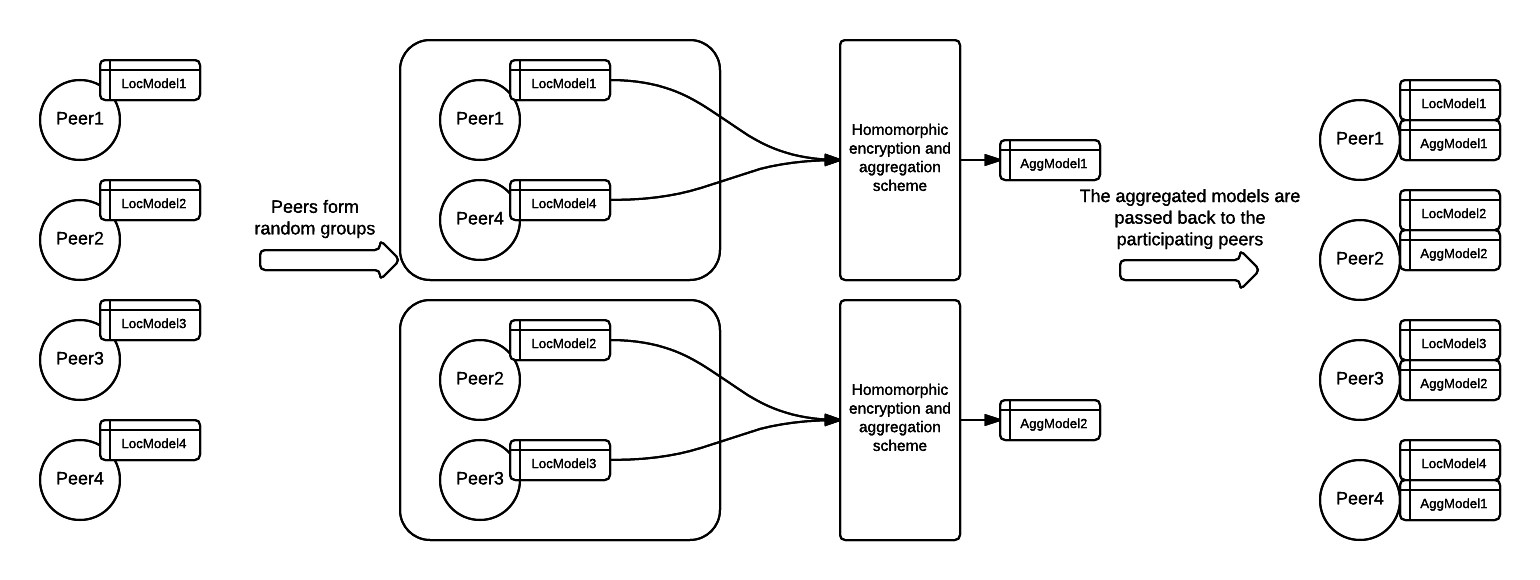
\includegraphics[width=\textwidth]{fig/peerModelCreation}
	\caption{One iteration of model aggregation}
	\label{fig:peerAggregationFigure}
\end{figure}


\subsection{Learning}
How is a logistic model implemented in our framework?

How is a model created and passed around the network?
Each Peer creates a logistic model based on their local data. They then form groups by calling the GroupFormingManager which assigns a group of peers together. This groups creates an aggregated model based on their own local ones. Here we simulate a Homomorphic Encryption scheme which assigns noise by secret sharing. 


How does the ensemble learning choose the best model?
What kind of performance metrics are used?
Mean classification error and Confusion Matrix.

\subsection{Privacy}
How does our framework guarantee differential privacy?
Based on the paper by 

\subsection{Experiment}
How are the experiments set up?
Explain the testing scheme.

Jade is re-run with while changing the initial parameters for the amount of peers, and the size of the groups they form. This test if performed over 10 iterations, while the mean classification error is recorded for each iteration. Each peer also create a confusion matrix with their classification results, and the peer with the best classification accuracy is saved and used to create a ROC-curve. 

Automatic testing scheme - Jade is configured so that it resets the main container after each experiment, and then re-run with new parameter configurations. 

Implemented 10-fold cross validation. This way we can tune the parameters and not be scared of our model overfitting on the test data. our initial solution was to use a single training and a single test set. This way we tuned the parameters so that they would give the best possible accuracy on the test set, which is not how the system should behave in the real world. 



\cleardoublepage